
\subsection{Arithmetic expression}\label{sec:expression}

In order to define arithmetic expressions involving real numbers  $\mathbb{R}$ in a rigorous way, we need to use a sophisticated type theory.
However, in order to keep things simple and maintain clarity, we will start by using only production rules, but with certain semantic restrictions.
We will also begin with rational numbers $\mathbb{Q}$ to avoid the difficulties inside real numbers $\mathbb{R}$ .

\begin{definition}\label{def:arithmetic-expression}
    An arithmetic expression $a$ over $\mathbb{Q}$ is a structure given by the following production rules:
\begin{equation}\label{eq:productionrule}
\begin{aligned}
a &\longleftarrow x\\
a &\longleftarrow ( a + a )\\
a &\longleftarrow ( a - a )\\
a &\longleftarrow ( a \times a )\\
a &\longleftarrow ( a \div a )
\end{aligned}
\end{equation}
    where $x \in \mathbb{Q}$, and we denote this as $a \in \mathbb{E} \left [\mathbb{Q} \right ]$.
\end{definition}

During the production process, we can obtain both a string representation and a tree representation of arithmetic expression $a$,
where the two representations are equivalent.
For instance, the string representation of $a$ might be:

\begin{equation}
(((((1 \times 2) \times 2) - 1) \times (2 + 1)) - 6)\label{eq:equation}
\end{equation}

and the parsed syntax tree is depicted in Figure~\ref{fig:syntaxtree}.

\begin{figure}[ht]
\centering
\resizebox{0.2\textheight}{!}{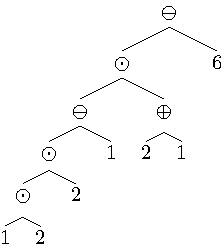
\includegraphics{images/02-example-expression-syntax-tree.pdf}}
\caption{a tree representation of an arithmetic expression}\label{fig:syntaxtree}\label{fig:figure}
\end{figure}

If we interpret the target as a string and the building processes in production rule~\eqref{eq:productionrule} as string building, we get the \emph{string representation}.
On the other hand, if the target is a tree, tree building leads to the \emph{tree representation}.
We can easily obtain the string representation of $a$ from its tree representation by performing a pre-order traversal.

The concept of a \emph{sub-expression} can also be derived from the concept of a subtree.
The branch nodes are all labeled with operators: $+$, $-$, $\times$, $\div$.
The leaf nodes are all labeled with numbers.

Evaluation $\nu$ is a partial function that operates on arithmetic expression $a \in \mathbb{E} \left [\mathbb{Q} \right ]$.
It is undefined only if division by zero occurs during the recursive evaluation process.

We can define evaluation $\nu(a)$ of $a$ recursively as follows:
\begin{itemize}
  \item Constant leaf: for any $x \in \mathbb{Q}$, $\nu(x) = x$.
  \item Compositional node by $+$: For any $(a + b)$, $\nu((a + b)) = \nu(a) + \nu(b)$.
  \item Compositional node by $-$: For any $(a - b)$, $\nu((a - b)) = \nu(a) - \nu(b)$.
  \item Compositional node by $\times$: For any $(a \times b)$, $\nu((a \times b)) = \nu(a) \nu(b)$.
  \item Compositional node by $\div$: For any $(a \div b)$, if $\nu(b) \neq 0$, then $\nu((a \div b)) = \nu(a) / \nu(b)$.
\end{itemize}

We say that an arithmetic expression $a$ is \emph{evaluable} if $\nu(a)$ is defined.
In the rest of this article, we will only consider evaluable arithmetic expressions unless stated otherwise.

Given an arithmetic expression $a$, whatever evaluable or not, we can obtain its tree representation.
If a node $l$ is a leaf node, its corresponding subexpression $s$ is a number, so we consider it to be already \("\)evaluated\("\).
If a node $b$ is a branch node, its corresponding subexpression $s$ is an expression, and we can apply $\nu$ to it to obtain a number $\nu(s)$.
During the recursive evaluation process, starting from the leaves and moving towards the root, the subexpressions are evaluated one after another.
However, the order of evaluations is generally not unique.

\begin{definition}
The evaluation order of an arithmetic expression $a$ is an ordering of branch nodes in the tree representation of $a$
such that every node (sub-expression) is evaluated before its parent.
\end{definition}

For example, the possible evaluation orders of the arithmetic expression in Figure~\ref{fig:syntaxtree} are:
\begin{itemize}
  \item $1 \times 2 \rightarrow \underline{2}; \underline{2} \times 2 \rightarrow \underline{4}; \underline{4} - 1 \rightarrow \underline{3}; 2 + 1 \rightarrow \underline{3}; \underline{3} \times \underline{3} \rightarrow \underline{9}; \underline{9} - 6 \rightarrow 3$
  \item $1 \times 2 \rightarrow \underline{2}; \underline{2} \times 2 \rightarrow \underline{4}; 2 + 1 \rightarrow \underline{3}; \underline{4} - 1 \rightarrow \underline{3}; \underline{3} \times \underline{3} \rightarrow \underline{9}; \underline{9} - 6 \rightarrow 3$
  \item $1 \times 2 \rightarrow \underline{2}; 2 + 1 \rightarrow \underline{3}; \underline{2} \times 2 \rightarrow \underline{4}; \underline{4} - 1 \rightarrow \underline{3}; \underline{3} \times \underline{3} \rightarrow \underline{9}; \underline{9} - 6 \rightarrow 3$
  \item $2 + 1 \rightarrow \underline{3}; 1 \times 2 \rightarrow \underline{2}; \underline{2} \times 2 \rightarrow \underline{4}; \underline{4} - 1 \rightarrow \underline{3}; \underline{3} \times \underline{3} \rightarrow \underline{9}; \underline{9} - 6 \rightarrow 3$
\end{itemize}

The underlined numbers are the numbers that are evaluated during the evaluation process.

Below are examples of expressions that have a unique evaluation order.
These include right-expanded, left-expanded,
and combinations of them, as shown in Figure~\ref{fig:leftright} and Figure~\ref{fig:combination}.

\begin{figure}[ht]
\centering
\resizebox{0.4\textheight}{!}{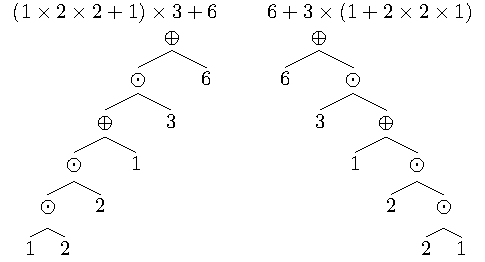
\includegraphics{images/03-example-expression-syntax-tree-left-right.pdf}}
\caption{right-expanded and left-expanded expressions}\label{fig:leftright}
\end{figure}

\begin{figure}[ht]
\centering
\resizebox{0.2\textheight}{!}{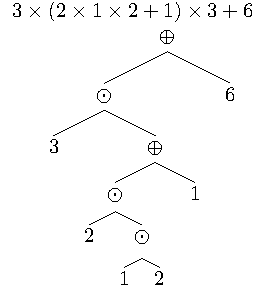
\includegraphics{images/04-example-expression-syntax-tree-combination}}
\caption{combinations of right-expanded and left-expanded expressions}\label{fig:combination}
\end{figure}

The evaluation order of an arithmetic expression is related to the topological order of its tree representation, but they are not the same.
The topological order of a tree is an ordering of nodes such that every node is visited before its parent\cite{Knuth1997TheAO}.
However, we are only interested in the ordering of branch nodes, as leaf nodes have already been evaluated and can be ignored.
Additionally, the topological order goes from parent to children, while the evaluation order goes from children to parent.

\begin{definition}
A threadlike expression is an arithmetic expression that all the left nodes in its tree representation are leaf nodes.
\end{definition}

So a threadlike expression is right-expanded and its evaluation order is unique.
One example of threadlike expressions is shown on the left side of Figure~\ref{fig:leftright}.

Threadlike expressions are significant here because they are analogous to the concept of paths in homotopy theory in geometry.
In a more general context, certain special types of threadlike expressions are also interesting:
for example, \emph{alternating threadlike expressions} are expressions in which the additional and multiplicative operators appear in an alternating manner.
In the field of computing, a hardware component called \emph{multiplier-accumulator} (MAC) unit has been implemented~\cite{Quinnell2007FloatingPointFM},
which is a special case of an alternating threadlike expression.
As a result, some numerical algorithms based on MAC units have been studied~\cite{Markstein2004SoftwareDA}.

\subsection{A scalar field and a mesh grid}\label{subsec:meshgrid}

Consider the upper half plane $\{\mathcal{H}: (x, y) | y > 0 \}$ equipped with an inner product and metrics defined as follows:

\[
\mathbf{a} \cdot \mathbf{b} = \begin{bmatrix} a_x & a_y \end{bmatrix} \begin{bmatrix} \frac{1}{y^2} & 0 \\ 0 & \frac{1}{y^2 \ln^2 2} \end{bmatrix} \begin{bmatrix} b_x \\ b_y \end{bmatrix}
\]

and

\[
ds^2 = \frac{1}{y^2} (dx^2 + \frac{dy^2}{\ln^2 2})
\]

We consider a scalar field satisfying

\begin{equation}
A = - \frac{x}{y}\label{eq:assignment}
\end{equation}

We call this field an \emph{assignment}.

Proper assignments allow us to establish a connection between paths in homotopy and threadlike arithmetic expressions,
and to incorporate function theory into the study of arithmetic expression geometry.

\begin{figure}[ht]
\centering
\resizebox{0.9\textwidth}{!}{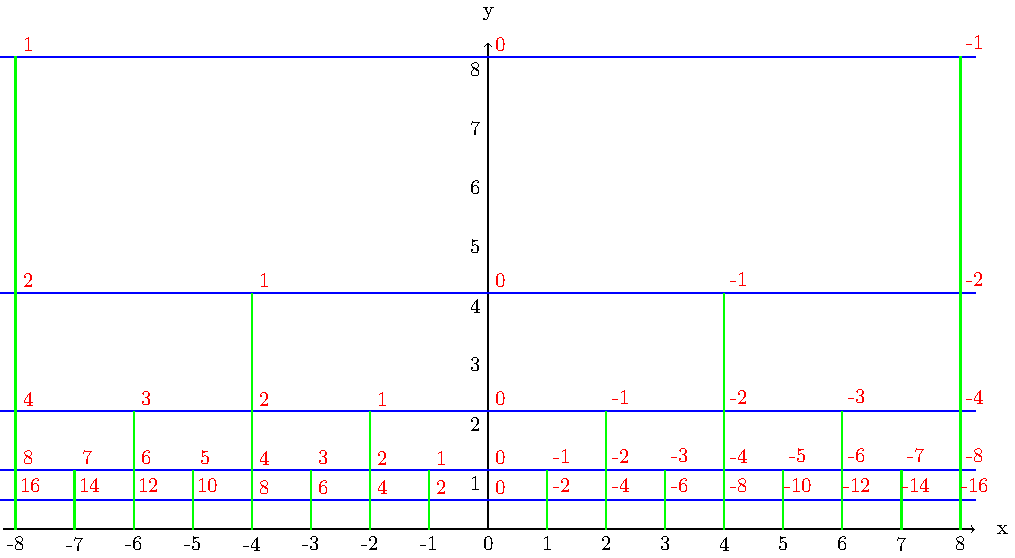
\includegraphics{images/01-grid-example-1.pdf}}
\caption{An addition-multiplication grid by generators with $\mu=1$ and $\lambda=\ln 2$}\label{fig:gridex0}
\end{figure}

We can draw a grid on the scalar field $A$ and underlying upper half plane $\mathcal{H}$ as shown in Figure~\ref{fig:gridex0}.
The blue lines encode a $+ 1$ relationship, the green lines encode a $\times 2$ relationship,
and they are line families that are perpendicular to each other.
The length of the line segments between two neighboring crossing points are unit length(calculations in lemma~\ref{lem:regular}).
The red value at the crossing points is the value of the scalar field $A$ at that point.
Based on the relationships encoded by the lines, we can encode threadlike arithmetic expressions,
which will be introduced in the subsection~\ref{subsec:encoding}.

The addition-multiplication grid is also scale-invariant under the transformation
\[
\begin{cases}
x' = \alpha x\\
y' = \alpha y
\end{cases}
\]

where $\alpha = 2^k , k \in \mathbb{Z}$.

We can imagine if we make the grid finer and finer, the grid will become a continuous space.
This leads to a rigorous treatment of arithmetic expressions as a geometric space in section~\ref{sec:topology}.

\subsection{Encoding threadlike expressions on the addition-multiplication grid}\label{subsec:encoding}

If we interpret the horizontal blue lines as $+ 1$ and the vertical green lines as $\times 2$ in Figure~\ref{fig:gridex0},
we can encode threadlike expressions on the addition-multiplication grid.
For example, in Figure~\ref{fig:encoding}
we encode $((((1 \times 4) - 1) \times 2) - 3)$ as the bold black lines.

\begin{figure}[ht]
\centering
\resizebox{0.9\textwidth}{!}{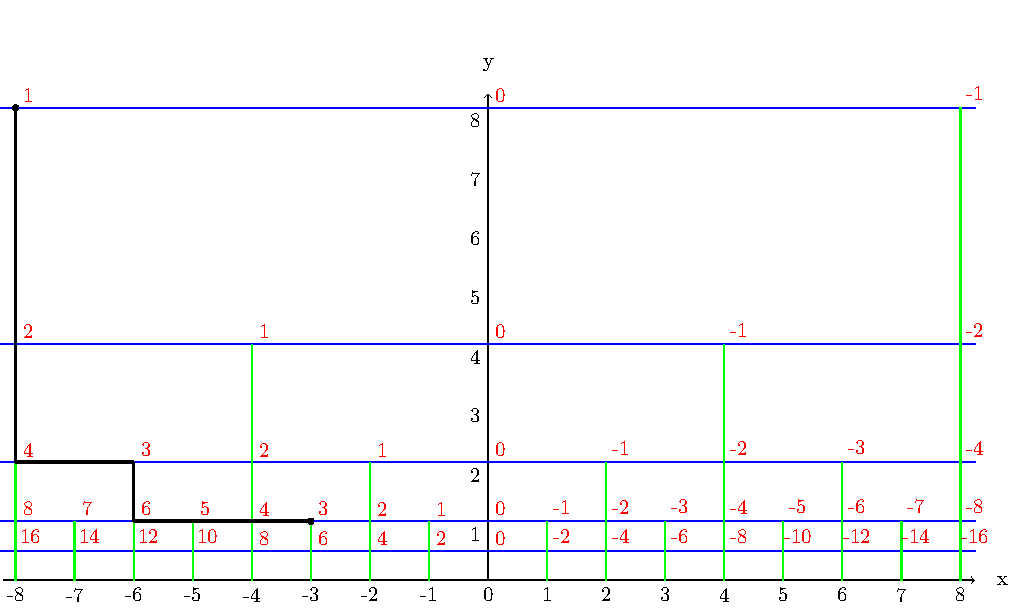
\includegraphics{images/05-example-expression-embedding}}
\caption{encoding threadlike expression}\label{fig:encoding}
\end{figure}

The zigzag lines in Figure~\ref{fig:encoding} can be divided into four parts:
\begin{itemize}
\item the vertical line from $1$ to $4$: encoded as multiplication by $4$
\item the horizontal line from $4$ to $3$: encoded as subtraction by $1$
\item the vertical line from $3$ to $6$: encoded as multiplication by $2$
\item the horizontal line from $6$ to $3$: encoded as subtraction by $3$
\end{itemize}

\subsection{From a scalar field to a space of threadlike expressions}\label{subsec:from-field-to-space}

As shown in Figure~\ref{fig:canonicalform}, we have the following paths and expressions:
\begin{itemize}
\item the black path: $((1 \times 8) - 5) = 3$
\item the purple path: $((1 - \frac{5}{8}) \times 8) = 3$
\item the brown path: $((((((1 - \frac{1}{8}) \times 2) - \frac{1}{2}) \times 2) - 1) \times 2) = 3$
\item the orange path: infinite many addition-multiplication terms accumulated together, a special kind of integration
\end{itemize}

\begin{figure}[ht]
\centering
\resizebox{0.9\textwidth}{!}{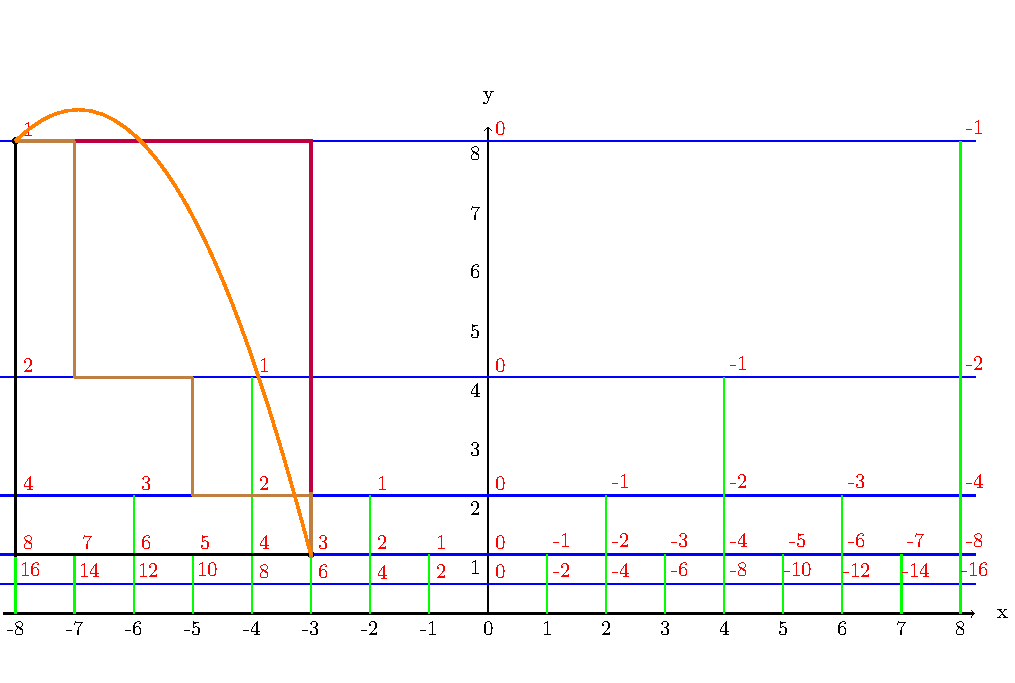
\includegraphics{images/06-example-canonical-form}}
\caption{different encodings and their canonical form}\label{fig:canonicalform}
\end{figure}

All of the paths in Figure~\ref{fig:canonicalform} have the same source $1$ and same target $3$.
We will discuss a canonical form for these paths.

It is easy to see that the expressions can be transformed into each other by using the multiplication distributive law and by combining and decomposing terms.

Conversion form brown path to black path
\begin{align}
3 & = ((((((1 - \frac{1}{8}) \times 2) - \frac{1}{2}) \times 2) - 1) \times 2) \\
& = 1 \times 8 -  \frac{1}{8} \times 8 - \frac{1}{2} \times 4 - 1 \times 2 \\
& = ((1 \times 8) - 5)
\end{align}

Conversion form brown path to purple path
\begin{align}
3 & = ((((((1 - \frac{1}{8}) \times 2) - \frac{1}{2}) \times 2) - 1) \times 2) \\
& = (1 - \frac{1}{8}) \times 8 - \frac{1}{2} \times 4 - 1 \times 2 \\
& = (1 - \frac{1}{8}) \times 8 - \frac{1}{4} \times 8 -  \frac{1}{4} \times 8 \\
& = (1 - \frac{1}{8} - \frac{1}{4} - \frac{1}{4}) \times 8 \\
& = ((1 - \frac{5}{8}) \times 8)
\end{align}

Therefore, we can define the black and purple paths in Figure~\ref{fig:canonicalform} as a pair of canonical paths,
which represent all threadlike expressions connecting the source $1$ and the target $3$.

Once we have such canonical paths, we can determine the canonical form of the whole space relative to an arbitrary source point $O$ and any other target point $P$.
This allows us to define the space as a space of threadlike expressions.
